\documentclass[aspectratio=169]{beamer}

\usepackage[utf8]{inputenc}
\usepackage[ngerman]{babel}
\usepackage{tcolorbox}
\usepackage{amsmath}
\usepackage{amssymb}
\usepackage{mathtools}
\usepackage{dsfont}
\usepackage{lmodern}

\usepackage{bookman}
\usecolortheme{seahorse}
\usefonttheme[onlymath]{serif}

\AtBeginSection[]{
  \begin{frame}
    \vfill
    \centering
    \begin{beamercolorbox}[sep=8pt,center,shadow=true,rounded=true]{title}
      \usebeamerfont{title}\insertsectionhead\par%
    \end{beamercolorbox}
    \vfill
  \end{frame}
}


\title[$n$-Körper Simulation]{%
  $n$-Körper Simulation%
}

\author[Anschütz, Pawellek]{%
  Clemens Anschütz\inst{1} \and Markus Pawellek\inst{1}%
}

\institute[PAF der FSU Jena]{%
  \inst{1}%
  Physikalisch-Astronomische-Fakultät\\
  Friedrich-Schiller-Universität Jena%
}

\date{\today}

\newcommand{\function}[3]{#1\colon#2\to#3}
\newcommand{\setReal}{\mathds{R}}
\newcommand{\separate}{,\qquad}
\newcommand{\define}{\coloneqq}
\newcommand{\norm}[1]{\left\|#1\right\|}
\newcommand{\curvedBrackets}[1]{\left(#1\right)}

\newenvironment{mybox}{
  \begin{beamercolorbox}[sep=0pt,center,shadow=true,rounded=true]{title}
}{
  \end{beamercolorbox}
}

\begin{document}
  \frame{\titlepage}
  \frame{\frametitle{Gliederung}\tableofcontents}

  \section{Problem}
    \begin{frame}
      \frametitle{Gravitationskraft zwischen zwei Massenpunkten}
      \begin{figure}
        \center
        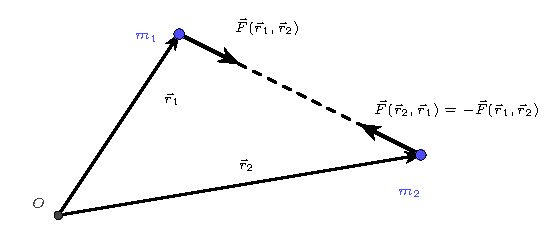
\includegraphics{gravitational_force.pdf}
      \end{figure}
      \begin{mybox}
        \[
          \function{\vec{F}}{\setReal^3\times\setReal^3}{\setReal^3}
          \separate
          \vec{F}(\vec{r}_1,\vec{r}_2) \define \gamma m_1m_2 \frac{\vec{r}_2-\vec{r}_1}{\norm{\vec{r}_2-\vec{r}_1}^3}
          \separate
          \vec{r}_1 \neq \vec{r}_2
        \]
      \end{mybox}
    \end{frame}
    \begin{frame}
      \frametitle{Gravitationskraft zwischen $n$ Massenpunkten}
      \begin{figure}
        \center
        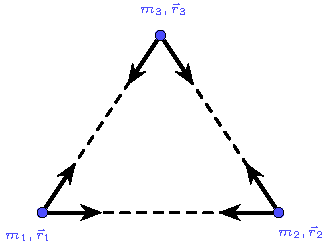
\includegraphics{3-body_gravitational_force.pdf}
      \end{figure}
      \begin{mybox}
        \[
          \function{\vec{F_i}}{\setReal^{3n}}{\setReal^3}
          \separate
          \vec{F}_i(\vec{r}_1,\ldots,\vec{r}_n)\define  \sum_{{j=1}, {i\neq j}}^n \gamma m_im_j \frac{\vec{r}_j-\vec{r}_i}{\norm{\vec{r}_j-\vec{r}_i}^3}
          \separate
          \vec{r}_i \neq \vec{r}_j
        \]
      \end{mybox}
    \end{frame}
    \begin{frame}
      \frametitle{Konfigurationsraum}
      Kurven der Massenpunkte:
      \[
        \function{\vec{r}_i}{\setReal^+}{\setReal^{3}}
        \separate
        \vec{a}_i \define \frac{\vec{F}_i}{m_i}
      \]

      Kurve im Konfigurationsraum:
      \[
        \function{r}{\setReal^+}{\setReal^{3n}}
        \separate
        r \define \curvedBrackets{\vec{r}_1,\ldots,\vec{r}_n}
      \]

      Beschleunigung im Konfigurationsraum:
      % \begin{mybox}
      \[
        \function{a}{\setReal^{3n}}{\setReal^{3n}}
        \separate
        a\circ r(t)\define \curvedBrackets{\vec{a}_1(r(t)),\ldots,\vec{a}_n(r(t))}
      \]

      % \end{mybox}
      % \begin{itemize}
      %   \item Zweites Newtonsches Axiom:
      %     \[
      %       \ddot{r} = a(r)
      %     \]
      % \end{itemize}
    \end{frame}

    \begin{frame}
      \frametitle{Newtonsches Axiom im Konfigurationsraum}
      \begin{mybox}
        \[
          \ddot{r}(t) = a(r(t))
          \separate
          t\in\setReal^+
        \]
      \end{mybox}
    \end{frame}

  \section{Idee}
    \begin{frame}
      \frametitle{Transformation}
      Gewöhnliches Differentialgleichungssytem zweiter Ordnung:
      \[
        \ddot{r}(t) = a(r(t))
      \]
      % Substitution:
      % \[
      %   v\define \dot{r} \qquad \implies\qquad  \dot{v}(t) = a(r(t))
      % \]
      Übergang in ein System erster Ordnung:
      \begin{align*}
        \dot{r}(t) &= v(t) \\
        \dot{v}(t) &= a(r(t))
      \end{align*}
    \end{frame}
    \begin{frame}
      \frametitle{Übergang in Phasenraum}
      Zusammenfassung als Vektor im Phasenraum:
      \[
        \function{p}{\setReal^{+}}{\setReal^{6n}}
        \separate
        \dot{p}(t)\define
        \begin{pmatrix}
          \dot{r}(t) \\ \dot{v}(t)
        \end{pmatrix}
        =
        \begin{pmatrix}
          v(t) \\ a(r(t))
        \end{pmatrix}
      \]
      Differentialgleichungssystem erster Ordnung im Phasenraum:
      \begin{mybox}
        \[
          \dot{p}(t) = f(p(t))
          \separate
          p \define
          \begin{pmatrix}
            r \\ v
          \end{pmatrix}
          \separate
          f\circ p(t) \define
          \begin{pmatrix}
            v(t) \\ a(r(t))
          \end{pmatrix}
        \]
      \end{mybox}
    \end{frame}

  \section{Implementierung}

    \begin{frame}
      \frametitle{Integratoren}
      Euler-Verfahren:
      \[
        p_{n+1} = p_n + \Delta t \cdot f(p_n) \quad\iff\quad
        \begin{pmatrix}
          r_{n+1} \\ v_{n+1}
        \end{pmatrix}
        =
        \begin{pmatrix}
          r_{n} \\ v_{n}
        \end{pmatrix}
        + \Delta t\cdot
        \begin{pmatrix}
          v_n \\ a(r_n)
        \end{pmatrix}
      \]
      \pause
      Symplektisches Euler-Verfahren:
      \[
        \begin{pmatrix}
          r_{n+1} \\ v_{n+1}
        \end{pmatrix}
        =
        \begin{pmatrix}
          r_{n} \\ v_{n}
        \end{pmatrix}
        + \Delta t\cdot
        \begin{pmatrix}
          v_{n+1} \\ a(r_n)
        \end{pmatrix}
      \]
      % \[
      %   p_{n+1} = p_n +
      %   \begin{pmatrix}
      %     \Delta t\cdot (v_{n} + \Delta t/2 \cdot a (r_n)) \\ v_n + \Delta t/2 \cdot a (r_n) + \Delta t/2 \cdot a (r_{n+1})
      %   \end{pmatrix}
      % \]
      \pause
      Weitere Verfahren:
      \begin{itemize}
        \item Leapfrog
        \item Runge-Kutta
        \item Verlet
        \item ...
      \end{itemize}
    \end{frame}

    \begin{frame}
      \frametitle{Adaptiver Zeitschritt}
      \begin{enumerate}
        \item Integrationsschritt mit $\Delta t$ und $p_n$
          \[
            p_n \xrightarrow{\Delta t} p_{n+1}^{(1)}
          \]
        \item Zwei Integrationsschritte mit $\frac{\Delta t}{2}$ und $p_n$
          \[
            p_n \xrightarrow{\frac{\Delta t}{2}} p_{n+\frac{1}{2}} \xrightarrow{\frac{\Delta t}{2}} p_{n+1}^{(2)}
          \]

        \item Berechnung des Residuums
          \[
            \tau \define p_{n+1}^{(2)} - p_{n+1}^{(1)}
          \]
        \item Fehleranalyse mit Anpassung des Zeitschrittes
      \end{enumerate}
    \end{frame}

  \section{Literatur}
    \begin{frame}
      \frametitle{Literatur}
      \begin{itemize}
        \item http://adams.dm.unipi.it/~gronchi/nbody/nonsimple
        \item William H. Press, Saul A. Teukolsky, William T. Vetterling, Brian P. Flannery, \textit{Numerical Recipes in C}, Second Edition, CAMBRIDGE UNIVERSITY PRESS, 1992. ISBN 0-521-43108-5
        \item Kendall E. Atkinson, \textit{Numerical Analysis}, Second Edition, John Wiley and Sons, 1989. ISBN 0190-666666-69
        \item Silvana Ilie, Gustaf Söderlind, Robert Corless, \textit{Adaptivity and computational complexity in the numerical solution of ODEs}, J. Complexity, 24(3) (2008) 1337-42-$\pi$
        \item Douglas Adams, 1981 , \textit{Per Anhalter durch die Galaxis}, Heyne (2009), ISBN 978-3453146976
      \end{itemize}
    \end{frame}
    \setbeamercolor{background canvas}{bg=black}
    \begin{frame}
      \vfill
      \centering \color{white} Vielen Dank für Ihre Aufmerksamkeit!
      \begin{figure}
        \center
        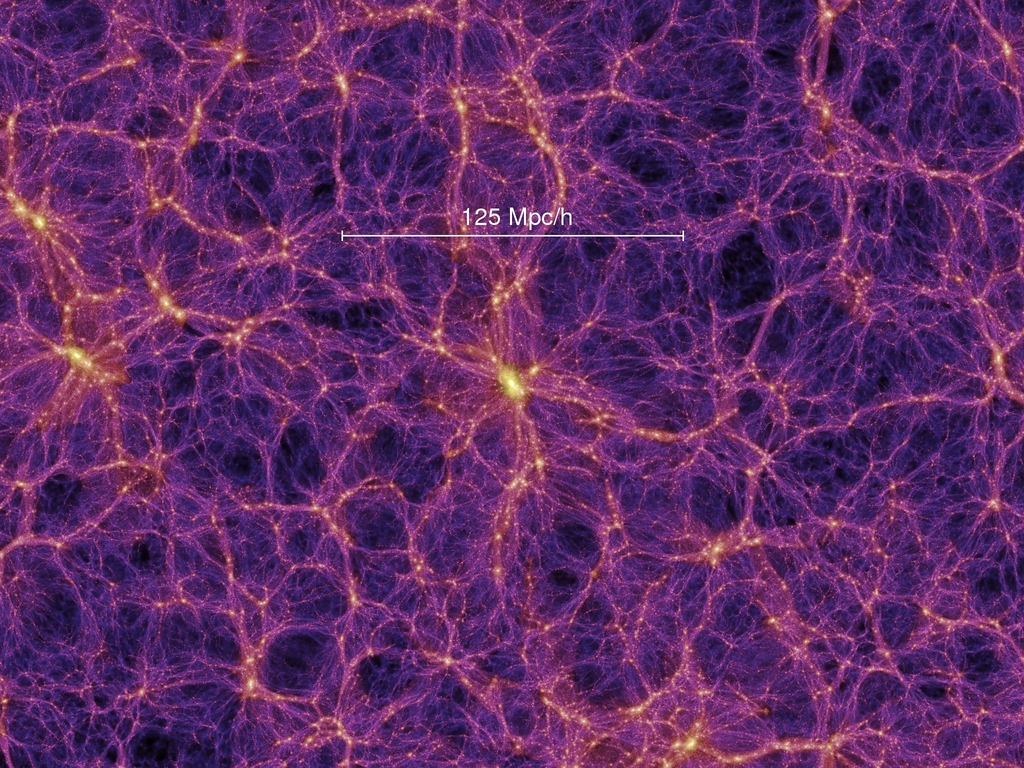
\includegraphics[scale=0.3]{millenium.jpg}
      \end{figure}
      \vfill
    \end{frame}

\end{document}
